\documentclass{article}

% if you need to pass options to natbib, use, e.g.:
%     \PassOptionsToPackage{numbers, compress}{natbib}
% before loading neurips_2019

% ready for submission
%\usepackage{neurips_2019_ml4ad}

% to compile a preprint version, e.g., for submission to arXiv, add add the
% [preprint] option:
 \usepackage[preprint]{neurips_2019_ml4ad}

% to compile a camera-ready version, add the [final] option, e.g.:
% \usepackage[final]{neurips_2019_ml4ad}

% to avoid loading the natbib package, add option nonatbib:
% \usepackage[nonatbib]{neurips_2019_ml4ad}

\usepackage[utf8]{inputenc} % allow utf-8 input
\usepackage[T1]{fontenc}    % use 8-bit T1 fonts
\usepackage{hyperref}       % hyperlinks
\usepackage{url}            % simple URL typesetting
\usepackage{booktabs}       % professional-quality tables
\usepackage{amsfonts}       % blackboard math symbols
\usepackage{nicefrac}       % compact symbols for 1/2, etc.
\usepackage{microtype}      % microtypography

% Custom packages
\usepackage{amsmath}
\usepackage{amssymb}
\usepackage{graphicx}
\usepackage{tikz}
\usepackage{float}
\usetikzlibrary{arrows,automata}
\usepackage{pgfplots}
\usetikzlibrary{intersections}

\title{Social Attention for Autonomous Decision-Making in Dense Traffic}

% The \author macro works with any number of authors. There are two commands
% used to separate the names and addresses of multiple authors: \And and \AND.
%
% Using \And between authors leaves it to LaTeX to determine where to break the
% lines. Using \AND forces a line break at that point. So, if LaTeX puts 3 of 4
% authors names on the first line, and the last on the second line, try using
% \AND instead of \And before the third author name.

%Happy Horizontal People Transporter
%From the Sirius Cybernetics Corporation with a Genuine People Personality

\author{%
  Edouard Leurent\thanks{Equal contribution.} \\
  Inria, SequeL team\\
  Renault Group\\
  Paris, France\\
  \texttt{edouard.leurent@renault.com} \\
  % examples of more authors
   \And
  Jean Mercat$^*$ \\
  Laboratoire des signaux et des syst\`emes,
  Centrale-Sup\'elec\\
  Renault Group\\
  Paris, France\\
  \texttt{jean.mercat@renault.com} \\
}

\begin{document}
	
	
	\tikzset{
		state/.style={
			rectangle,
			draw=black, very thick,
			minimum height=2em,
			inner sep=2pt,
			text centered,
		},
		name plot/.style={every path/.style={name path global=#1}}
	}
	
	\pgfmathdeclarefunction{dnorm}{2}{%
		\pgfmathparse{1/(#2*sqrt(2*pi))*exp(-((x-#1)^2)/(2*#2^2))}%
	}
	

\maketitle

\begin{abstract}
  The abstract paragraph should be indented \nicefrac{1}{2}~inch (3~picas) on
  both the left- and right-hand margins. Use 10~point type, with a vertical
  spacing (leading) of 11~points.  The word \textbf{Abstract} must be centered,
  bold, and in point size 12. Two line spaces precede the abstract. The abstract
  must be limited to one paragraph.
\end{abstract}

\section{Introduction}

Automated Decision Making
Modular pipeline: perception, high level representation, decision: behaviour planning, trajectory, control
large litterature on perception
trajectory optimization and control is well understood

behaviour planning by rule-based systems, fsm
but behaviour planning is difficult, complex scenes, in particular interactions with other drivers difficult to model explicitly.
 -> leverage (deep) learning method
Learning from demonstration: nice results for lane keeping, not so much for interaction, also require costly demonstration . 

Conversely, leverage simulation:
Reinforcement learning:
Framing as an MDP, choose a good representation.
List of vehicles with their coordinates 
but variable size, + combinatorial representation
Occupancy grid / images : fixed size, tradeoff:  low accuracy vs exploding size

\section{Background and Related Work}

\subsection{Model-Free Deep Reinforcement Learning}

- MDP
- Value function
- DQN

\subsection{State Representation for Social Interactions}
In the state:
Kinematics
Not fixed size
Occupancy grid

In the model:

Weight sharing ?

\section{Model Architecture}

Motivation: 
\begin{enumerate}
	\item Out of a complex scene description, the model should be able to filter information and consider only what is relevant for decision. In other words, the agent should \emph{pay attention} to vehicles that are close or conflict with the planned route;
	\item The model should be able to admit a variable number of vehicles as inputs;
	\item The model should be invariant to the ordering of vehicles.
\end{enumerate}


\begin{figure}[ht]
	\centering
	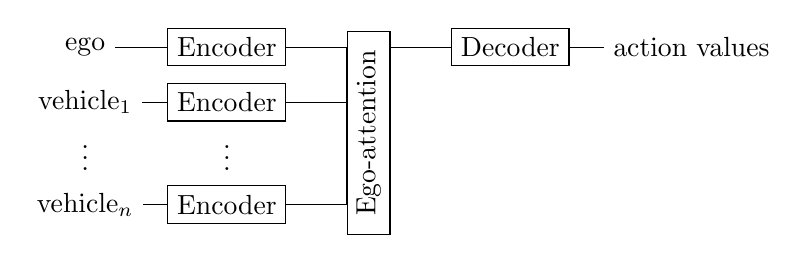
\begin{tikzpicture}
	\node(X1){ego};
	\node[below of=X1, node distance=0.7cm](X2){vehicle$_{1}$};
	\node[below of=X2, node distance=0.6cm](X3){$\vdots$};
	\node[below of=X3, node distance=0.7cm](X4){vehicle$_{n}$};
	
	\node[draw, right of=X1, node distance=1.8cm, rectangle](ENC1){Encoder};
	\node[draw, right of=X2, node distance=1.8cm, rectangle](ENC2){Encoder};
	\node[below of=ENC2, node distance=0.6cm](ENC3){$\vdots$};
	\node[draw, right of=X4, node distance=1.8cm, rectangle](ENC4){Encoder};
	
	\path (X1) edge (ENC1);
	\path (X2) edge (ENC2);
	\path (X4) edge (ENC4);
	
	
	\node[draw, rectangle, right of=ENC1, node distance=1.8cm, below=-0.2cm](TRANS1){\rotatebox{90}{ Ego-attention }};
	
	\draw (ENC1.east) -| (TRANS1.west);
	\draw (ENC2.east) -| (TRANS1.west);
	\draw (ENC4.east) -| (TRANS1.west);
	
	
	\node[draw, right of=ENC1, node distance=3.6cm, rectangle](DEC1){Decoder};
	
	\draw (TRANS1.east) |- (DEC1.west);

	\node[right of=DEC1, node distance=2.3cm](Y1){action values};
	
	\draw (DEC1.east) -- (Y1.west);
	
	%        \draw[decorate,decoration={brace,mirror}] (X1.north west) -- node[left=10pt] {$X$} (X3.south west);
	\end{tikzpicture}
	\caption{Block diagram of our model architecture.}
	\label{sch_whole_model}
	
\end{figure}


The multi-head self-attention layers allow vehicle interactions while keeping independence from their number
and ordering.
This mechanism is described in~\cite{Vaswani2017} where it is applied on sentence translation.
In this section we explain its use for vehicle interactions.
The computations made by each attention head is represented on figure~\ref{fig:ego-attention} and are detailed below.

\begin{figure}[ht]
	\centering
	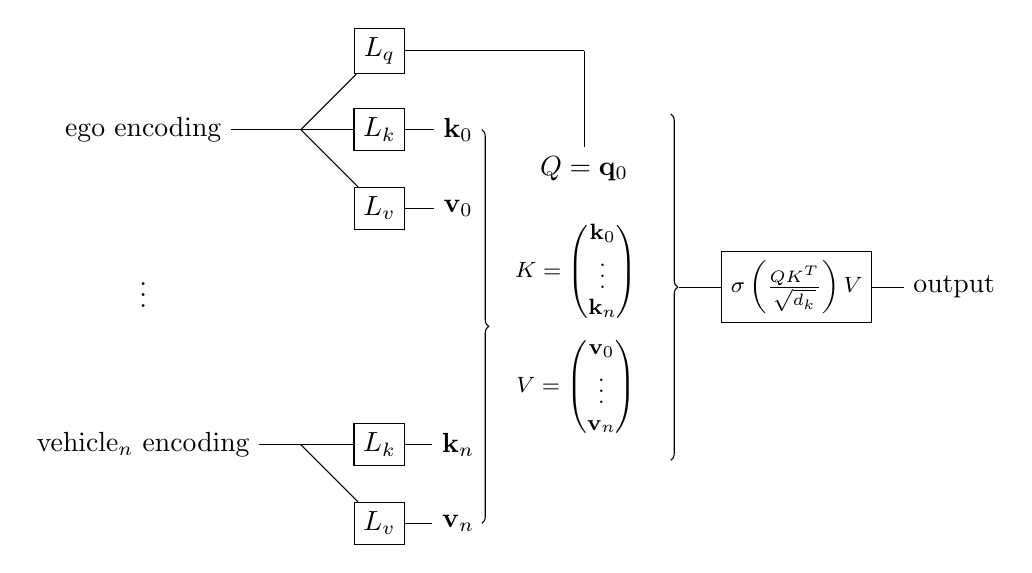
\begin{tikzpicture}[scale=1, every node/.style={scale=1}]
	\node(X1){ego encoding};
	\node[below of=X1, node distance=2cm](X2){$\vdots$};
	\node[below of=X2, node distance=2cm](X3){vehicle$_{n}$ encoding};
	
	\coordinate[right of= X1, node distance=2cm](X1b){};
	
	\draw (X1) -- (X1b);
	
	\node[draw, right of=X1b, node distance=1cm](LK1){$L_{k}$};
	\node[draw, below of=LK1, node distance=1cm](LV1){$L_{v}$};
	\node[draw, above of=LK1, node distance=1cm](LQ1){$L_{q}$};
	
	\draw (X1b) -- (LQ1);
	\draw (X1b) -- (LK1);
	\draw (X1b) -- (LV1);
	
	\coordinate[right of=LQ1, node distance=2.6cm](Q1){};
	\node[below of=Q1, node distance=1.5cm](Q2){$Q = \mathbf{q}_0$};
	\node[right of=LK1, node distance=1cm](K1){$\mathbf{k}_0$};
	\node[right of=LV1, node distance=1cm](V1){$\mathbf{v}_0$};
	
	\draw (LQ1) -- (Q1);
	\draw (Q1) -- (Q2);
	\draw (LK1) -- (K1);
	\draw (LV1) -- (V1);
	
	\coordinate[right of= X3, node distance=2cm](X3b){};
	
	\draw (X3) -- (X3b);
	
	\node[draw, right of=X3b, node distance=1cm](LK3){$L_{k}$};
	\node[draw, below of=LK3, node distance=1cm](LV3){$L_{v}$};

	\draw (X3b) -- (LK3);	
	\draw (X3b) -- (LV3);
	
	\node[right of=LK3, node distance=1cm](K3){$\mathbf{k}_{n}$};
	\node[right of=LV3, node distance=1cm](V3){$\mathbf{v}_{n}$};

	\draw (LK3) -- (K3);
	\draw (LV3) -- (V3);
	
	\coordinate[right of=K1, node distance=0.3cm](TOP){};
	\coordinate[right of=V3, node distance=0.3cm](BOT){};
	\draw[decorate,decoration={brace}] (TOP) -- node[left=5pt]{} (BOT);
	
	\node[right of=X2, text width=3cm, node distance=5.5cm, below=-1.0cm](EQ){\footnotesize \[K = \left( \begin{matrix}
		\mathbf{k}_0 \\
		\vdots \\
		\mathbf{k}_{n}
		\end{matrix} \right)\]
		\\
		\footnotesize \[ V = \left( \begin{matrix}
		\mathbf{v}_0 \\
		\vdots \\
		\mathbf{v}_{n}
		\end{matrix}\right) \]
	};

	\node[draw, right of=X2, node distance=8.3cm](EQ2){
	\footnotesize $\sigma\left(\frac{QK^T}{\sqrt{d_k}}\right)V$};

	\coordinate[left of=EQ2, node distance=1.6cm, above=2.2cm](TOP2){};
	\coordinate[left of=EQ2, node distance=1.5cm, below=0.0cm](MID2){};
	\coordinate[left of=EQ2, node distance=1.6cm, below=2.2cm](BOT2){};
	\draw[decorate,decoration={brace}] (TOP2) -- node[left=5pt]{} (BOT2);
	\draw (MID2) -- (EQ2);
	
	\node[right of=EQ2, node distance=2cm](OUT){output};
	\draw (EQ2) -- (OUT);
	
	\end{tikzpicture}
	\caption{Architecture of an ego-attention head.
		The blocks $L_{q}$, $L_{k}$, $L_{v}$ are linear layers. The keys $K$ and values $V$ are concatenated from all vehicles, while the query $Q$ is only produced by the ego-vehicle.}
	\label{fig:ego-attention}
\end{figure}

Each vehicle should pay attention to specific features from a selection of the other vehicles.
This is made with four steps: pulling together specific features, identifying these feature collections,
enquiring among identifiers, and gathering the results.
Each head produces a different selection of features using a linear projection of
the input tensor resulting in the value tensor $V$.
To identify these features, a key tensor $K$ is associated to each value.
Then, each vehicle must select which other vehicle to pay attention to.
For that purpose a query $Q$ is produced to find a selection of keys.
The match score between a key and a query is the dot product is scaled with the square root of the key
dimension $\sqrt{d_k}$ and normalized with a softmax.
This produces an attention matrix that contains coefficients close to $1$ for matching queries and keys
and close to $0$ otherwise.
Finally, this matrix is used to gather the values from $V$.
Thus, the self-attention computation for each head is written:
\begin{equation}
\text{output}=\underbrace{\sigma\left(\frac{QK^T}{\sqrt{d_k}}\right)}_{\text{attention matrix}}V
\label{eq_selfattention}
\end{equation}
The outputs from all heads are concatenated and combined with a linear layer.
The resulting tensor is then added to the input as in residual networks.


\section{Experiments}
\subsection{The intersection task}

We consider a situation where interactions between vehicles is important: crossing an unsignalized intersection.

To that end, we use the highway-env environment and propose a novel intersection task.

- The intersection: cross (North/South/East/West), single lane or 2 lane ?
- The other vehicles: are spawned randomly, and plan a route to a random direction.
Follow a Kinematic Bicycle Model, lane keeping with a low-level steering controller, longitudinal control with IDM


\subsection{The baselines}
\subsection{Performances}
\subsection{Attention interpretation}

Additional videos are available at \url{http://url.github.io}

\section{Conclusion}

\subsubsection*{Acknowledgments}

Use unnumbered third level headings for the acknowledgments. All acknowledgments
Go at the end of the paper. Do not include acknowledgments in the anonymized
submission, only in the final paper.

\section*{References}



\end{document}
